\subsection{CWMP}

\gls{cwmp}, also known as \gls{tr069}, was introduced in 2004 with the intention of defining the communication between a \gls{cpe} and an \gls{acs} \cite{tr069}. \gls{cwmp} is commonly used by \glspl{isp} to manage residential gateways remotely, without requiring user intervention. The placement of the protocol in the infrastructure is shown on Figure \ref{figure:tr069_figure1}.

\begin{figure}[h]
    \centering
    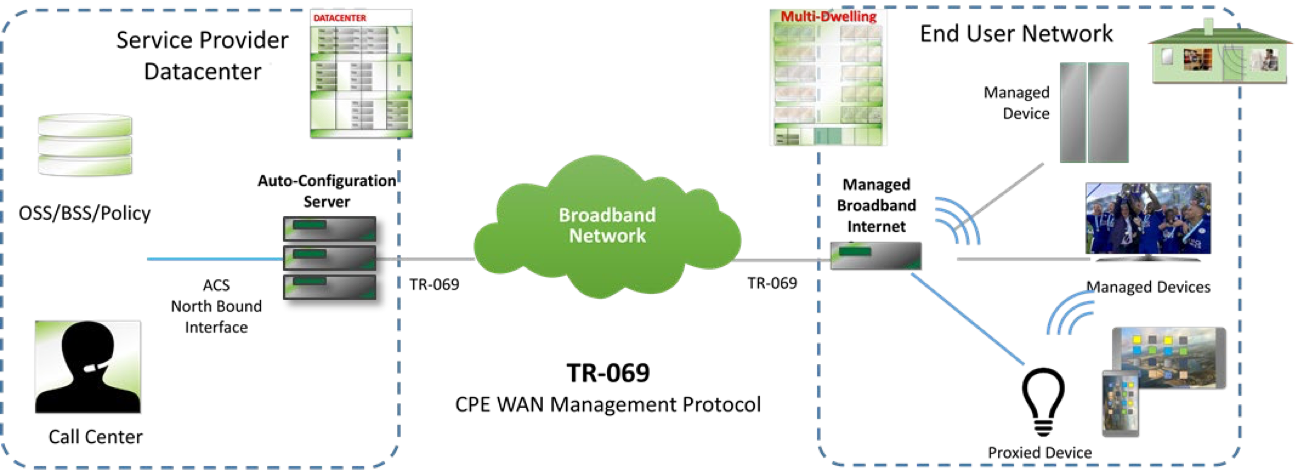
\includegraphics[width=\linewidth]{contents/background-in-isp-side-protocols/cwmp/positioning-in-the-e2e-architecture.png}
    \caption{Positioning in the End-to-End Architecture}
    {Source: \cite{tr069}}
    \label{figure:tr069_figure1}
\end{figure}

\glspl{cpe} can be provisioned as soon as they connect to the broadband access network and can be re-configured at any time by the \gls{acs}. The provides mechanisms for the \gls{cpe} to download software and firmware updates, self-initiated or \gls{acs}-initiated, notifying the \gls{acs} upon success or failure. Software can be installed, updated, uninstalled, enabled, or disabled on the \gls{cpe} via \gls{cwmp}. The \gls{acs} may monitor the \gls{cpe}'s status and performance, also being able to run diagnostic tests and collect the results.

\FloatBarrier
